\documentclass[11pt,a4paper]{article}
\usepackage[utf8]{inputenc}
\usepackage[T1]{fontenc}
\usepackage{amsmath,amssymb,amsfonts}
\usepackage{amsthm}
\usepackage[margin=2.5cm]{geometry}
\usepackage{enumitem}
\usepackage{tikz}
\usepackage{xcolor}
\usepackage{hyperref}
\hypersetup{colorlinks=true,linkcolor=blue!55!black,urlcolor=blue!55!black}
\setlist[itemize]{leftmargin=1.4em,itemsep=2pt,topsep=3pt}

% ── theorem environments (numbered, standard) ──
\newtheorem{theorem}{Theorem}[section]
\newtheorem{lemma}[theorem]{Lemma}
\newtheorem{proposition}[theorem]{Proposition}
\newtheorem{corollary}[theorem]{Corollary}
\theoremstyle{definition}
\newtheorem{definition}[theorem]{Definition}
\newtheorem{example}[theorem]{Example}
\newtheorem{remark}[theorem]{Remark}
\newtheorem{exercise}{Exercise}

% ── macros (all safe, multi-character) ──
\newcommand{\Z}{\mathbb{Z}}
\newcommand{\Q}{\mathbb{Q}}
\newcommand{\R}{\mathbb{R}}
\newcommand{\C}{\mathbb{C}}
\newcommand{\F}{\mathbb{F}}
\newcommand{\GL}{\operatorname{GL}}
\newcommand{\SL}{\operatorname{SL}}
\newcommand{\SO}{\operatorname{SO}}
\newcommand{\Aut}{\operatorname{Aut}}
\newcommand{\Inn}{\operatorname{Inn}}
\newcommand{\Sym}{\operatorname{Sym}}
\newcommand{\im}{\operatorname{im}}
\newcommand{\ord}{\operatorname{ord}}
\newcommand{\id}{\operatorname{id}}
\newcommand{\Gal}{\operatorname{Gal}}
\newcommand{\Orb}{\operatorname{Orb}}
\newcommand{\Stab}{\operatorname{Stab}}

\title{
	{\color{blue!40!black}\textbf{\Huge Point}}\\[0.3em]
	\Large \textit{From Number Theory to Algebraic Geometry and Logic}\\[0.7em]
	\large \textbf{Session P1 --- Group Theory: Part I}\\[0.3em]
	\normalsize \emph{Complete lecture notes with proofs, examples, and exercises}
}
\author{}
\date{}

\begin{document}
	\maketitle
	\thispagestyle{empty}
	
	\begin{abstract}
		\noindent
		This is the entry session of the course. It builds the language of \emph{symmetry} --- groups,
		subgroups, quotients, and actions --- which will reappear as Galois groups (Act~II), ideal class
		groups (S24), idele class groups (S49), fundamental groups (P3, S35), and automorphism groups of
		logical structures (Act~VII). Every structural result used later is proved here: the subgroup
		criterion, Lagrange's theorem and its corollaries, the injectivity criterion via kernels, the
		well-definedness of quotient groups, the three isomorphism theorems, and the Orbit--Stabilizer
		theorem. The session closes with the philosophical pattern the course will instantiate again and
		again: \emph{a quotient is what remains when viewpoints that look the same are identified}.
	\end{abstract}
	
	\subsection*{Session plan (150 minutes)}
	\begin{center}\small
		\begin{tabular}{|l|l|}
			\hline
			\textbf{Time} & \textbf{Block} \\
			\hline
			0:00--0:10 & Orientation: symmetry as the engine of the course; where groups return \\
			0:10--0:30 & \S1 Groups: definition, examples, cancellation \\
			0:30--0:55 & \S2 Subgroups; the criterion; cyclic groups; Lagrange and corollaries \\
			0:55--1:05 & \emph{Break} \\
			1:05--1:25 & \S3 Homomorphisms; kernels; injectivity; centers and inner automorphisms \\
			1:25--1:55 & \S4 Normal subgroups; quotients; the three isomorphism theorems; three worked examples \\
			1:55--2:20 & \S5 Actions; Orbit--Stabilizer; conjugation and the class equation; Cayley \\
			2:20--2:30 & Wrap-up: the quotient philosophy; bridge to P2--P3 and Act~II \\
			\hline
		\end{tabular}
	\end{center}
	
	\subsection*{Conventions}
	Groups are written multiplicatively with identity $e$ unless stated otherwise; $\Z$, $\Z/n\Z$,
	$\Q$, $\R$, $\C$ are additive unless a $\times$ or $*$ is displayed. For a subset $S$ of a group,
	$S^{-1}=\{s^{-1}:s\in S\}$. All homomorphisms send $e$ to $e$ (proved, not assumed).
	
	\tableofcontents
	\newpage
	
	% ══════════════════════════════════════════════
	\section{Groups: Definition and First Examples}
	% ══════════════════════════════════════════════
	
	\begin{definition}[Group]
		A \textbf{group} is a set $G$ with a binary operation $G\times G\to G$, $(g,h)\mapsto gh$, such that:
		\begin{enumerate}[label=(G\arabic*)]
			\item \emph{Associativity:} $(gh)k=g(hk)$ for all $g,h,k\in G$;
			\item \emph{Identity:} there exists $e\in G$ with $eg=ge=g$ for all $g$;
			\item \emph{Inverses:} for each $g$ there exists $g^{-1}$ with $gg^{-1}=g^{-1}g=e$.
		\end{enumerate}
		The group is \textbf{abelian} if $gh=hg$ for all $g,h$. Its \textbf{order} is $|G|$ (possibly $\infty$).
	\end{definition}
	
	\begin{lemma}[Uniqueness and housekeeping]\label{lem:basics}
		In any group: the identity is unique; each inverse is unique; $(gh)^{-1}=h^{-1}g^{-1}$;
		$(g^{-1})^{-1}=g$; and $eg=g$ together with $hg=g$ already force $h=e$.
	\end{lemma}
	\begin{proof}
		If $e,e'$ are identities then $e=ee'=e'$. If $x,x'$ invert $g$ then
		$x=xe=x(gx')=(xg)x'=ex'=x'$. Now $h^{-1}g^{-1}$ is an inverse of $gh$ since
		$(gh)(h^{-1}g^{-1})=g(hh^{-1})g^{-1}=gg^{-1}=e$ and similarly on the other side; uniqueness gives
		$(gh)^{-1}=h^{-1}g^{-1}$. Taking $g=h^{-1}$ in $(gh)^{-1}=h^{-1}g^{-1}$ gives $(g^{-1})^{-1}=g$.
		Finally $hg=g=eg$ implies $h=e$ by left-cancelling $g$ (multiply by $g^{-1}$ on the right).
	\end{proof}
	
	\begin{proposition}[Cancellation laws]
		$gh=gk\Rightarrow h=k$ and $hg=kg\Rightarrow h=k$.
	\end{proposition}
	\begin{proof}
		Multiply $gh=gk$ on the left by $g^{-1}$.
	\end{proof}
	
	\begin{example}[Running examples]\label{ex:groups}
		\begin{itemize}
			\item $(\Z,+)$, $(\Q,+)$, $(\R,+)$, $(\C,+)$: infinite abelian.
			\item $(\Q^*,\times)$, $(\R^*,\times)$, $(\C^*,\times)$: units; abelian.
			\item $(\Z/n\Z,+)$: finite abelian of order $n$.
			\item The \textbf{circle group} $U(1)=\{z\in\C^*:|z|=1\}$ under multiplication; abelian; the group of rotations of the plane.
			\item The \textbf{symmetric group} $S_n=\Sym(\{1,\dots,n\})$ under composition; non-abelian for $n\ge3$; $|S_n|=n!$.
			\item $\GL_n(k)=\{A\in M_n(k):\det A\neq0\}$ under multiplication; non-abelian for $n\ge2$;
			$\SL_n(k)=\{A:\det A=1\}$; $\SO_n(\R)=\{A\in\SL_n(\R):A^{\mathsf T}A=I\}$ (rotations of $\R^n$).
			\item Direct products $G\times H$ with componentwise operation.
			\item The trivial group $\{e\}$.
		\end{itemize}
		Every new notion in this session should be tested on all of these.
	\end{example}
	
	\begin{remark}[Why groups, why here]
		A group is ``all the symmetries of an object, packaged''. The course will meet: symmetries of field
		extensions (Galois groups, Act~II), symmetries of coverings (P3, S35), symmetries of lattices and
		curves (Acts~III--V), and symmetries of logical theories (Act~VII). The machinery below is the
		common grammar.
	\end{remark}
	
	% ══════════════════════════════════════════════
	\section{Subgroups, Cyclic Groups, and Lagrange}
	% ══════════════════════════════════════════════
	
	\begin{definition}[Subgroup]
		$H\subseteq G$ is a \textbf{subgroup}, written $H\le G$, if $e\in H$, $H$ is closed under the
		operation, and $H$ is closed under inverses. Equivalently $H$ is a group with the restricted law.
	\end{definition}
	
	\begin{proposition}[Subgroup criterion]\label{prop:subgroup}
		A nonempty subset $H\subseteq G$ is a subgroup $\iff$ for all $x,y\in H$ one has $xy^{-1}\in H$.
	\end{proposition}
	\begin{proof}
		($\Rightarrow$) Clear. ($\Leftarrow$) Take $x=y$: $e=xx^{-1}\in H$. Then for $y\in H$,
		$y^{-1}=ey^{-1}\in H$. Then for $x,y\in H$, $xy=x(y^{-1})^{-1}\in H$. So $H$ satisfies the definition.
	\end{proof}
	
	\begin{example}
		$\Z\le\Q\le\R\le\C$ (additive); $\SL_n(k)\le\GL_n(k)$; $\SO_n(\R)\le\GL_n(\R)$; $U(1)\le\C^*$;
		$n\Z\le\Z$; and $\{e\}\le G\le G$ always. Non-example: $\Z_{\ge0}\subseteq\Z$ (no inverses);
		$\{0,2,4\}\subseteq\Z/6\Z$ \emph{is} a subgroup (check the criterion), of order $3$.
	\end{example}
	
	\begin{definition}[Generated and cyclic subgroups]
		For $S\subseteq G$, the \textbf{subgroup generated by $S$} is
		$\langle S\rangle=\bigcap\{H\le G:S\subseteq H\}$, the smallest subgroup containing $S$.
		For one element, $\langle g\rangle$ makes $G$ (or the subgroup) \textbf{cyclic} if $G=\langle g\rangle$
		for some $g$; such $g$ is a \textbf{generator}.
	\end{definition}
	
	\begin{proposition}\label{prop:generated}
		$\langle S\rangle$ equals the set of all finite products of elements of $S\cup S^{-1}$; in particular
		$\langle g\rangle=\{g^n:n\in\Z\}$, and every cyclic group is abelian.
	\end{proposition}
	\begin{proof}
		The set of finite products of $S\cup S^{-1}$ contains $S$ (length-one products), contains $e$ (empty
		product), and is closed under product and inverse, hence is a subgroup containing $S$; conversely any
		subgroup containing $S$ contains all such products. For $S=\{g\}$ this gives $\{g^n\}$. Commutativity:
		$g^mg^n=g^{m+n}=g^ng^m$.
	\end{proof}
	
	\begin{definition}[Order of an element]
		$\ord(g)=|\langle g\rangle|$; equivalently the smallest $n\ge1$ with $g^n=e$, and $\infty$ if none.
	\end{definition}
	
	\begin{proposition}\label{prop:order}
		If $\ord(g)=n<\infty$ then $g^k=e\iff n\mid k$, and $\langle g\rangle=\{e,g,\dots,g^{n-1}\}$ has
		exactly $n$ elements. If $\ord(g)=\infty$ then all $g^k$, $k\in\Z$, are distinct.
	\end{proposition}
	\begin{proof}
		Write $k=qn+r$, $0\le r<n$; then $g^k=(g^n)^q g^r=g^r$, so $g^k=e\Rightarrow g^r=e\Rightarrow r=0$ by
		minimality of $n$. Distinctness of $e,g,\dots,g^{n-1}$: if $g^i=g^j$ with $0\le j<i<n$ then
		$g^{i-j}=e$ with $0<i-j<n$, contradiction. The infinite case is the same argument with no $n$.
	\end{proof}
	
	\begin{definition}[Cosets and index]
		For $H\le G$ and $g\in G$, the \textbf{left coset} is $gH=\{gh:h\in H\}$; the set of left cosets is
		$G/H$; the \textbf{index} is $[G:H]=|G/H|$.
	\end{definition}
	
	\begin{lemma}\label{lem:cosets}
		Left cosets partition $G$, and each has the same cardinality as $H$.
	\end{lemma}
	\begin{proof}
		$g\in gH$ since $e\in H$, so cosets cover $G$. If $gH\cap g'H\neq\varnothing$ then $gh=g'h'$, so
		$g=g'h'h^{-1}$ and $gH\subseteq g'H$; symmetrically $g'H\subseteq gH$, so overlapping cosets coincide:
		a partition. The map $H\to gH$, $h\mapsto gh$, is bijective with inverse $x\mapsto g^{-1}x$.
	\end{proof}
	
	\begin{theorem}[Lagrange]\label{thm:lagrange}
		If $G$ is finite and $H\le G$ then $|H|$ divides $|G|$, and $|G|=[G:H]\cdot|H|$.
	\end{theorem}
	\begin{proof}
		$G$ is the disjoint union of $[G:H]$ cosets, each of size $|H|$ (Lemma~\ref{lem:cosets}); sum the sizes.
	\end{proof}
	
	\begin{corollary}\label{cor:lagrange}
		For finite $G$:
		\begin{enumerate}[label=(\alph*)]
			\item $\ord(g)$ divides $|G|$ for every $g\in G$;
			\item $g^{|G|}=e$ for every $g$;
			\item a group of prime order $p$ is cyclic, generated by any $g\neq e$;
			\item the only subgroups of $\Z/p\Z$ are $\{0\}$ and itself.
		\end{enumerate}
	\end{corollary}
	\begin{proof}
		(a) $\ord(g)=|\langle g\rangle|$ divides $|G|$ by Lagrange applied to $\langle g\rangle$.
		(b) $g^{|G|}=g^{\ord(g)\cdot(|G|/\ord(g))}=e$. (c) Any $g\neq e$ has $\ord(g)\mid p$ and $\ord(g)>1$,
		so $\ord(g)=p$ and $\langle g\rangle=G$. (d) Immediate from (c) and Lagrange.
	\end{proof}
	
	\begin{example}
		Subgroups of $\Z/12\Z$: one for each divisor, of orders $1,2,3,4,6,12$; element orders likewise divide
		$12$. In $S_3$ (order $6$): element orders are $1,2,3$ only. In $\F_p^*$ (order $p-1$):
		$a^{p-1}=1$ for all $a\neq0$ --- this is Fermat's little theorem, obtained purely from Lagrange.
	\end{example}
	
	\begin{remark}[The converse of Lagrange fails]\label{rem:converse}
		$A_4$ has order $12$ but \emph{no} subgroup of order $6$ (Exercise~\ref{ex:a4}). The correct
		converse-direction statements are Sylow's theorems (mention; not needed later) and, in the course,
		the Galois correspondence (S13), which repairs the converse for \emph{Galois} groups.
	\end{remark}
	
	\begin{figure}[h]
		\centering
		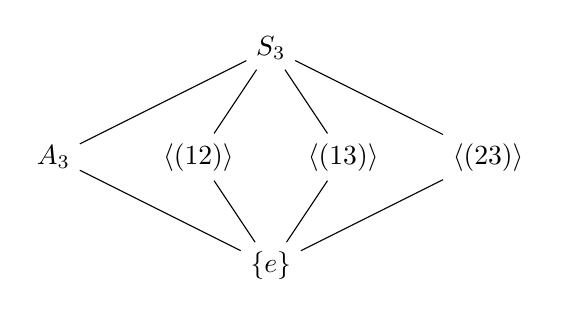
\begin{tikzpicture}[scale=1.15]
			\node (top) at (0,2.4) {$S_3$};
			\node (a3) at (-2.4,1.2) {$A_3$};
			\node (h1) at (-0.8,1.2) {$\langle(12)\rangle$};
			\node (h2) at (0.8,1.2) {$\langle(13)\rangle$};
			\node (h3) at (2.4,1.2) {$\langle(23)\rangle$};
			\node (bot) at (0,0) {$\{e\}$};
			\draw (top) -- (a3); \draw (top) -- (h1); \draw (top) -- (h2); \draw (top) -- (h3);
			\draw (a3) -- (bot); \draw (h1) -- (bot); \draw (h2) -- (bot); \draw (h3) -- (bot);
		\end{tikzpicture}
		\caption{The subgroup lattice of $S_3$: six subgroups, orders $1,2,2,2,3,6$ --- all dividing $6$, as
			Lagrange demands. Exactly one of the proper nontrivial ones ($A_3$) will turn out to be normal
			(\S4).}
	\end{figure}
	
	% ══════════════════════════════════════════════
	\section{Homomorphisms, Kernels, and Centers}
	% ══════════════════════════════════════════════
	
	\begin{definition}[Homomorphism]
		$\varphi:G\to H$ is a \textbf{homomorphism} if $\varphi(gh)=\varphi(g)\varphi(h)$ for all $g,h$.
		Its \textbf{kernel} is $\ker\varphi=\{g\in G:\varphi(g)=e_H\}$ and its \textbf{image}
		$\im\varphi=\varphi(G)$.
	\end{definition}
	
	\begin{proposition}\label{prop:hom-basics}
		$\varphi(e_G)=e_H$; $\varphi(g^{-1})=\varphi(g)^{-1}$; $\ker\varphi\le G$; $\im\varphi\le H$.
	\end{proposition}
	\begin{proof}
		$\varphi(e)=\varphi(ee)=\varphi(e)\varphi(e)$, cancel $\varphi(e)$. Then
		$e=\varphi(e)=\varphi(gg^{-1})=\varphi(g)\varphi(g^{-1})$ gives inverses. Subgroup criterion:
		$e\in\ker$; if $\varphi(x)=\varphi(y)=e$ then $\varphi(xy^{-1})=ee=e$. Same for $\im$ with products
		and inverses in $H$.
	\end{proof}
	
	\begin{theorem}[Injectivity criterion]\label{thm:injective}
		$\varphi$ is injective $\iff\ker\varphi=\{e_G\}$.
	\end{theorem}
	\begin{proof}
		($\Rightarrow$) $\varphi(e)=e$, so injectivity forces $\ker=\{e\}$. ($\Leftarrow$) If
		$\varphi(g)=\varphi(h)$ then $e=\varphi(g)\varphi(h)^{-1}=\varphi(gh^{-1})$, so $gh^{-1}\in\ker=\{e\}$,
		hence $g=h$.
	\end{proof}
	
	\begin{definition}[Isomorphism; automorphism; center; inner automorphisms]
		An \textbf{isomorphism} is a bijective homomorphism ($G\cong H$). An \textbf{automorphism} is an
		isomorphism $G\to G$; they form $\Aut(G)$. For $g\in G$, conjugation $c_g(x)=gxg^{-1}$ is an
		automorphism, called \textbf{inner}; the \textbf{center} is $Z(G)=\{g:gh=hg\ \forall h\}$.
	\end{definition}
	
	\begin{proposition}
		$c_g\in\Aut(G)$; the map $g\mapsto c_g$ is a homomorphism $G\to\Aut(G)$ with kernel $Z(G)$; hence
		$Z(G)\le G$ and the inner automorphisms form a subgroup $\Inn(G)\le\Aut(G)$.
	\end{proposition}
	\begin{proof}
		$c_g(xy)=gxg^{-1}gyg^{-1}=c_g(x)c_g(y)$; bijective with inverse $c_{g^{-1}}$. $c_{gh}=c_g\circ c_h$ is
		direct. $c_g=\id\iff gx=xg\ \forall x\iff g\in Z(G)$, so the kernel is $Z(G)$; kernels are subgroups
		(Proposition~\ref{prop:hom-basics}), and the image $\Inn(G)$ is a subgroup of $\Aut(G)$.
	\end{proof}
	
	\begin{example}\label{ex:homs}
		\begin{itemize}
			\item $\det:\GL_n(k)\to k^*$ is a surjective homomorphism; $\ker\det=\SL_n(k)$.
			\item \textbf{The sign homomorphism} $\operatorname{sign}:S_n\to\{\pm1\}$: let
			$\Delta=\prod_{i<j}(x_i-x_j)\in\Z[x_1,\dots,x_n]$; $\sigma\in S_n$ permutes the variables and sends
			each factor to $\pm$ a factor, so $\sigma(\Delta)=\pm\Delta$; define $\sigma(\Delta)=\operatorname{sign}(\sigma)\Delta$.
			Then $(\sigma\tau)(\Delta)=\sigma(\tau(\Delta))$ gives multiplicativity; a transposition swaps one
			pair and fixes the parity of the rest, hence has sign $-1$. Kernel $=A_n$ (defined as $\ker$).
			\item $\exp:(\R,+)\to(\R_{>0},\times)$ is an isomorphism with inverse $\log$.
			\item Reduction $\pi:\Z\to\Z/n\Z$ is surjective with kernel $n\Z$.
			\item $Z(\GL_n(k))=\{\lambda I:\lambda\in k^*\}$; $Z(S_n)=\{e\}$ for $n\ge3$ (exercises).
		\end{itemize}
	\end{example}
	
	% ══════════════════════════════════════════════
	\section{Normal Subgroups, Quotients, and the Isomorphism Theorems}
	% ══════════════════════════════════════════════
	
	\begin{definition}[Normal subgroup]
		$N\le G$ is \textbf{normal}, $N\trianglelefteq G$, if $gNg^{-1}=N$ for all $g\in G$.
	\end{definition}
	
	\begin{proposition}[Equivalent criteria]\label{prop:normal}
		For $N\le G$ the following are equivalent:
		\begin{enumerate}[label=(\alph*)]
			\item $gNg^{-1}=N$ for all $g$;
			\item $gNg^{-1}\subseteq N$ for all $g$;
			\item $gN=Ng$ for all $g$ (left cosets $=$ right cosets);
			\item $N$ is a union of conjugacy classes $\{gng^{-1}:n\in N\}\subseteq N$ pointwise-generated.
		\end{enumerate}
	\end{proposition}
	\begin{proof}
		(a)$\Rightarrow$(b) trivial. (b)$\Rightarrow$(a): apply (b) to $g^{-1}$: $g^{-1}Ng\subseteq N$, so
		$N\subseteq gNg^{-1}$, and with (b) equality. (a)$\Leftrightarrow$(c): $gN=Ng\iff gNg^{-1}=N$ by
		multiplying on the right by $g^{-1}$. (d) is a restatement of (b).
	\end{proof}
	
	\begin{proposition}[Kernels are normal; and only kernels]\label{prop:kernel-normal}
		$\ker\varphi\trianglelefteq G$ for any homomorphism $\varphi$; conversely every normal subgroup is
		the kernel of the projection constructed in Theorem~\ref{thm:quotient}.
	\end{proposition}
	\begin{proof}
		$\varphi(gng^{-1})=\varphi(g)\varphi(n)\varphi(g)^{-1}=e$, so $g\ker g^{-1}\subseteq\ker$; apply
		Proposition~\ref{prop:normal}(b).
	\end{proof}
	
	\begin{example}
		In abelian groups every subgroup is normal. $A_n\trianglelefteq S_n$ and $\SL_n\trianglelefteq
		\GL_n$ as kernels. $\Z(G)\trianglelefteq G$. Non-example: $\langle(12)\rangle\le S_3$ is \emph{not}
		normal: $(13)(12)(13)^{-1}=(23)\notin\langle(12)\rangle$ --- compare Figure~1: normality is rare.
	\end{example}
	
	\begin{theorem}[Quotient groups]\label{thm:quotient}
		Let $N\trianglelefteq G$. On the coset set $G/N$ the rule
		\[
		(gN)\cdot(hN):=(gh)N
		\]
		is well defined and makes $G/N$ a group; the projection $\pi:G\to G/N$, $g\mapsto gN$, is a
		surjective homomorphism with $\ker\pi=N$; and $|G/N|=[G:N]$.
	\end{theorem}
	\begin{proof}
		Well-definedness: if $g'=gn_1$, $h'=hn_2$ then
		$g'h'N=gn_1hn_2N=g h (h^{-1}n_1 h)n_2 N=ghN$ since $h^{-1}n_1h\in N$ by normality and $N N=N$.
		Associativity inherits from $G$; identity $eN=N$; inverse $(gN)^{-1}=g^{-1}N$. $\pi$ is a
		homomorphism by the very definition of the product; $\pi(g)=N\iff gN=N\iff g\in N$.
	\end{proof}
	
	\begin{theorem}[First Isomorphism Theorem]\label{thm:first-iso}
		For $\varphi:G\to H$ a homomorphism, the map
		\[
		\bar\varphi:G/\ker\varphi\longrightarrow\im\varphi,\qquad g\ker\varphi\longmapsto\varphi(g)
		\]
		is a well-defined isomorphism; in particular $G/\ker\varphi\cong\im\varphi$.
	\end{theorem}
	\begin{proof}
		Well-defined: if $g'=gk$, $k\in\ker$, then $\varphi(g')=\varphi(g)\varphi(k)=\varphi(g)$. Homomorphism:
		inherited. Injective: $\bar\varphi(g\ker)=e\Rightarrow\varphi(g)=e\Rightarrow g\ker=\ker$. Surjective
		onto $\im\varphi$ by definition.
	\end{proof}
	
	\begin{example}[Three worked applications]\label{ex:first-iso}
		\begin{enumerate}[label=(\roman*)]
			\item $\det:\GL_n(k)\twoheadrightarrow k^*$, $\ker=\SL_n(k)$ $\Rightarrow$
			$\GL_n(k)/\SL_n(k)\cong k^*$. Over $k=\F_q$: $|\SL_n(\F_q)|=|\GL_n(\F_q)|/(q-1)$.
			\item $\operatorname{sign}:S_n\twoheadrightarrow\{\pm1\}$, $\ker=A_n$ $\Rightarrow$
			$S_n/A_n\cong\Z/2$, hence $|A_n|=n!/2$.
			\item $\pi:\Z\twoheadrightarrow\Z/n\Z$, $\ker=n\Z$ $\Rightarrow$ $\Z/n\Z\cong\Z/n\Z$ (tautological but
			canonical); more usefully: any homomorphism $\Z\to G$ is $1\mapsto g$, kernel $\ord(g)\Z$, so
			$\Z/\ord(g)\Z\cong\langle g\rangle$ --- \emph{every cyclic group is a quotient of $\Z$}.
		\end{enumerate}
	\end{example}
	
	\begin{theorem}[Second and Third Isomorphism Theorems]\label{thm:second-third}
		Let $G$ be a group.
		\begin{enumerate}[label=(\alph*)]
			\item \emph{(Second)} If $H\le G$ and $N\trianglelefteq G$ then $HN=\{hn\}\le G$, $N\trianglelefteq HN$,
			$H\cap N\trianglelefteq H$, and $HN/N\cong H/(H\cap N)$.
			\item \emph{(Third)} If $N\trianglelefteq G$ and $N\subseteq H\trianglelefteq G$ then
			$H/N\trianglelefteq G/N$ and $(G/N)/(H/N)\cong G/H$.
		\end{enumerate}
	\end{theorem}
	\begin{proof}
		(a) $HN$ is a subgroup because $N$ normal: $(h_1n_1)(h_2n_2)=h_1h_2(h_2^{-1}n_1h_2)n_2\in HN$, and
		inverses similarly. Define $\psi:H\to HN/N$ by $\psi(h)=hN$; this is a homomorphism (restriction of
		$\pi$), surjective since $hnN=hN$, and $\ker\psi=\{h:h\in N\}=H\cap N$; apply
		Theorem~\ref{thm:first-iso}. (b) The map $G/N\to G/H$, $gN\mapsto gH$, is a well-defined surjective
		homomorphism (well-defined since $N\subseteq H$) with kernel $\{gN:g\in H\}=H/N$; apply
		Theorem~\ref{thm:first-iso}.
	\end{proof}
	
	\begin{remark}[The quotient philosophy]\label{rem:quotient-philosophy}
		$G/N$ is what you see of $G$ when you declare everything in $N$ invisible. The First Isomorphism
		Theorem says: \emph{every} homomorphic image of $G$ arises this way, and the kernel records exactly
		what was blurred. This is the group-theoretic prototype of: norm groups blurring ideles in Artin
		reciprocity (S47--S49), residue fields blurring local rings (S1, S28), and models identifying
		provably equal terms (Act~VII). Quotients are \emph{spaces of viewpoints collapsed to points}.
	\end{remark}
	
	% ══════════════════════════════════════════════
	\section{Group Actions, Orbits, and the Class Equation}
	% ══════════════════════════════════════════════
	
	\begin{definition}[Action]
		A \textbf{(left) action} of $G$ on a set $X$ is a map $G\times X\to X$, $(g,x)\mapsto g\cdot x$, with
		$e\cdot x=x$ and $g\cdot(h\cdot x)=(gh)\cdot x$.
	\end{definition}
	
	\begin{proposition}\label{prop:action-hom}
		Actions of $G$ on $X$ are in bijection with homomorphisms $\rho:G\to\Sym(X)$, via
		$\rho(g)(x)=g\cdot x$.
	\end{proposition}
	\begin{proof}
		Given an action, each $\rho(g)$ is bijective with inverse $\rho(g^{-1})$, and $\rho(gh)=\rho(g)\rho(h)$
		is the action axiom; so $\rho$ is a homomorphism. Conversely a homomorphism defines an action by
		$g\cdot x:=\rho(g)(x)$; the two constructions invert each other.
	\end{proof}
	
	\begin{example}\label{ex:actions}
		\begin{itemize}
			\item $S_n$ on $\{1,\dots,n\}$ (tautological); on $k$-element subsets; on ordered tuples.
			\item $\GL_n(k)$ on $k^n$ by matrix multiplication; on lines through the origin (projective space).
			\item \textbf{Conjugation:} $G$ on itself, $g\cdot x=gxg^{-1}$; and on its subgroups, $g\cdot H=gHg^{-1}$
			(normal subgroups $=$ fixed points of this action).
			\item \textbf{Left multiplication:} $G$ on itself, $g\cdot x=gx$ (free and transitive).
			\item $D_4$ (symmetries of the square) on its four vertices; rotation subgroup on vertices.
			\item Trivial action $g\cdot x=x$ for all $g$.
		\end{itemize}
	\end{example}
	
	\begin{definition}[Orbit, stabilizer, fixed points]
		$\Orb(x)=\{g\cdot x:g\in G\}$; $\Stab(x)=\{g:g\cdot x=x\}\le G$; $X^G=\{x:g\cdot x=x\ \forall g\}$.
		The action is \textbf{transitive} if there is one orbit, \textbf{free} if all stabilizers are trivial.
	\end{definition}
	
	\begin{theorem}[Orbit--Stabilizer]\label{thm:orbit-stabilizer}
		The map $G/\Stab(x)\to\Orb(x)$, $g\Stab(x)\mapsto g\cdot x$, is a well-defined bijection; hence for
		finite $G$,
		\[
		|G|=|\Orb(x)|\cdot|\Stab(x)|.
		\]
	\end{theorem}
	\begin{proof}
		Well-defined: $g'=gs$ with $s\in\Stab(x)$ gives $g'\cdot x=g\cdot(s\cdot x)=g\cdot x$. Injective:
		$g\cdot x=g'\cdot x\Rightarrow g^{-1}g'\cdot x=x\Rightarrow g^{-1}g'\in\Stab(x)\Rightarrow g\Stab=g'\Stab$.
		Surjective: by definition of orbit. Counting: $|G/\Stab(x)|=[G:\Stab(x)]=|G|/|\Stab(x)|$ by Lagrange.
	\end{proof}
	
	\begin{example}[Computing orders via Orbit--Stabilizer]
		\begin{itemize}
			\item $S_n$ on $\{1,\dots,n\}$: orbit of $1$ has size $n$; $\Stab(1)\cong S_{n-1}$; inductively
			$|S_n|=n\cdot(n-1)!$ --- Lagrange-free derivation of $n!$.
			\item $\GL_n(\F_q)$ on $\F_q^n\setminus\{0\}$: orbit is everything (transitive), stabilizer of $e_1$
			has $q^{n-1}(q^{n-1}-1)\cdots$ --- cleanly: $|\GL_n(\F_q)|=(q^n-1)(q^n-q)\cdots(q^n-q^{n-1})$ by
			choosing columns (exercise, both ways).
			\item $D_4$ on vertices: orbit size $4$, stabilizer of a vertex has order $2$, so $|D_4|=8$.
		\end{itemize}
	\end{example}
	
	\begin{proposition}[Class equation]\label{prop:class-equation}
		For finite $G$, partitioning $G$ into conjugacy classes (orbits of the conjugation action), with
		representatives $x_i$ of the non-singleton classes:
		\[
		|G|=|Z(G)|+\sum_i [G:C_G(x_i)],\qquad C_G(x)=\Stab_{\text{conj}}(x)=\{g:gx=xg\}.
		\]
	\end{proposition}
	\begin{proof}
		Orbits of the conjugation action partition $G$; singleton orbits are exactly central elements;
		non-singleton orbits have size $[G:C_G(x_i)]$ by Orbit--Stabilizer. Sum orbit sizes.
	\end{proof}
	
	\begin{theorem}[Cayley]\label{thm:cayley}
		Every group $G$ embeds into $\Sym(G)$; in particular every finite group of order $n$ is isomorphic to
		a subgroup of $S_n$.
	\end{theorem}
	\begin{proof}
		The left-multiplication action gives $\rho:G\to\Sym(G)$ (Proposition~\ref{prop:action-hom});
		$\ker\rho=\{g:gx=x\ \forall x\}=\{e\}$ (take $x=e$), so $\rho$ is injective by
		Theorem~\ref{thm:injective}.
	\end{proof}
	
	\begin{remark}[Where actions return]\label{rem:actions-return}
		Galois groups act on roots and on intermediate fields (S12--S13); $\pi_1$ acts on fibers of coverings
		(P3, S35); Frobenius elements act on points of varieties mod $p$ (S9, S40, S46); automorphism groups
		act on models of theories (Act~VII). Orbit--Stabilizer is the counting engine behind all of these,
		and the class equation is the seed of the simplicity proof for $A_n$ (S11).
	\end{remark}
	
	% ══════════════════════════════════════════════
	\section{Exercises}
	% ══════════════════════════════════════════════
	\begin{exercise}
		Prove that the intersection of any family of subgroups is a subgroup, and that $\langle S\rangle$ as
		defined by intersection equals the set of finite products of $S\cup S^{-1}$.
	\end{exercise}
	\begin{exercise}
		List all subgroups of $\Z/12\Z$ and of $S_3$; draw both lattices; identify which are cyclic and which
		are normal.
	\end{exercise}
	\begin{exercise}
		Show that a nonempty finite subset $H$ of a group closed under the operation is already a subgroup
		(finiteness is essential: find a counterexample in $(\Z,+)$).
	\end{exercise}
	\begin{exercise}
		Prove: if $G$ is a group in which $g^2=e$ for all $g$, then $G$ is abelian. More generally, if
		$(gh)^2=g^2h^2$ for all $g,h$, then $G$ is abelian.
	\end{exercise}
	\begin{exercise}
		Prove $\operatorname{sign}$ as defined in Example~\ref{ex:homs} is a well-defined homomorphism and
		that a transposition has sign $-1$. Conclude $|A_n|=n!/2$.
	\end{exercise}
	\begin{exercise}
		Show $Z(\GL_n(k))=\{\lambda I:\lambda\in k^*\}$ and $Z(S_n)=\{e\}$ for $n\ge3$.
	\end{exercise}
	\begin{exercise}
		Give an explicit homomorphism $\varphi:\Z\to\Z$ with $\im\varphi=6\Z$; then describe
		$\Z/\ker\varphi$ and check the First Isomorphism Theorem by hand.
	\end{exercise}
	\begin{exercise}
		In $S_4$, take $H=\langle(12)\rangle$ and $N=\{e,(12)(34),(13)(24),(14)(23)\}$ (check $N\trianglelefteq S_4$).
		Verify the Second Isomorphism Theorem: compute $HN$, $H\cap N$, and both sides of $HN/N\cong H/(H\cap N)$.
	\end{exercise}
	\begin{exercise}\label{ex:a4}
		Prove $A_4$ has no subgroup of order $6$ (hint: such a subgroup would be normal of index $2$; look at
		the three double transpositions). This shows the converse of Lagrange fails.
	\end{exercise}
	\begin{exercise}
		Using Orbit--Stabilizer, compute $|\GL_n(\F_q)|$ in two ways: (i) by choosing a basis column by
		column; (ii) via the action on $\F_q^n\setminus\{0\}$ and induction on the stabilizer.
	\end{exercise}
	\begin{exercise}
		Write the class equation of $S_4$ explicitly (conjugacy classes $=$ cycle types) and verify the sum.
	\end{exercise}
	\begin{exercise}
		Let $G$ act on $X$. Prove that orbits partition $X$, and that the action is transitive $\iff$
		$X\cong G/\Stab(x)$ as $G$-sets for any $x$.
	\end{exercise}
	
	% ══════════════════════════════════════════════
	\section*{Where This Session Feeds the Course}
	\addcontentsline{toc}{section}{Where This Session Feeds the Course}
	% ══════════════════════════════════════════════
	\begin{itemize}
		\item \textbf{Depends on:} nothing --- this is the entry point of the course.
		\item \textbf{Feeds:} Act~II entirely (Galois groups, simplicity of $A_n$ via the class equation,
		solvability); S24 (ideal class group as a quotient group); S47--S49 (Artin reciprocity as a First
		Isomorphism Theorem at global scale: $C_K/N(C_L)\cong\Gal(L/K)$); P3 and S35 (deck transformations
		and \'etale $\pi_1$ as permutation groups of fibers); Act~VII (automorphism groups of models).
		\item \textbf{Unifying thread:} a quotient group is a space of viewpoints collapsed to points; a
		group action is a family of points moving under symmetry; kernels record exactly what an
		evaluation (homomorphism) cannot see.
	\end{itemize}
	
	\subsection*{References for this session}
	\begin{enumerate}[label={[\arabic*]}]
		\item Artin, M. \emph{Algebra}, ch.2.
		\item Herstein, I.N. \emph{Topics in Algebra}, ch.2.
		\item Rotman, J.J. \emph{An Introduction to the Theory of Groups}, ch.1--4.
		\item Dummit, D. \& Foote, R. \emph{Abstract Algebra}, ch.1--4 (supplementary, rich exercises).
		\item Lang, S. \emph{Algebra}, ch.I (supplementary).
	\end{enumerate}
	
	\vspace{1.5em}
	\begin{center}
		\rule{0.6\textwidth}{0.4pt}\\[0.5em]
		\textit{End of Session P1 --- next: Session P2, Topology and Metric Spaces}
	\end{center}
	
\end{document}